% Template file for an a0 landscape poster.
% Written by Graeme, 2001-03 based on Norman's original microlensing
% poster.
%
% See discussion and documentation at
% <http://www.astro.gla.ac.uk/users/norman/docs/posters/> 
%
% $Id: poster-template-landscape.tex,v 1.2 2002/12/03 11:25:46 norman Exp $


% Default mode is landscape, which is what we want, however dvips and
% a0poster do not quite do the right thing, so we end up with text in
% landscape style (wide and short) down a portrait page (narrow and
% long). Printing this onto the a0 printer chops the right hand edge.
% However, 'psnup' can save the day, reorienting the text so that the
% poster prints lengthways down an a0 portrait bounding box.
%
% 'psnup -w85cm -h119cm -f poster_from_dvips.ps poster_in_landscape.ps'

\documentclass[a0]{a0poster}
% You might find the 'draft' option to a0 poster useful if you have
% lots of graphics, because they can take some time to process and
% display. (\documentclass[a0,draft]{a0poster})
\input defs
\pagestyle{empty}
\setcounter{secnumdepth}{0}
\renewcommand{\familydefault}{\sfdefault}
\newcommand{\QED}{~~\rule[-1pt]{8pt}{8pt}}\def\qed{\QED}

\renewcommand{\reals}{{\mbox{\bf R}}}

% The textpos package is necessary to position textblocks at arbitary 
% places on the page.
\usepackage[absolute]{textpos}

\usepackage{fleqn,psfrag,wrapfig,tikz}

\usepackage[papersize={38in,28in}]{geometry}

% Graphics to include graphics. Times is nice on posters, but you
% might want to switch it off and go for CMR fonts.
\usepackage{graphics}


% we are running pdflatex, so convert .eps files to .pdf
%\usepackage[pdftex]{graphicx}
%\usepackage{epstopdf}

% These colours are tried and tested for titles and headers. Don't
% over use color!
\usepackage{color}
\definecolor{Red}{rgb}{0.9,0.0,0.1}

\definecolor{bluegray}{rgb}{0.15,0.20,0.40}
\definecolor{bluegraylight}{rgb}{0.35,0.40,0.60}
\definecolor{gray}{rgb}{0.3,0.3,0.3}
\definecolor{lightgray}{rgb}{0.7,0.7,0.7}
\definecolor{darkblue}{rgb}{0.2,0.2,1.0}
\definecolor{darkgreen}{rgb}{0.0,0.5,0.3}

\renewcommand{\labelitemi}{\textcolor{bluegray}\textbullet}
\renewcommand{\labelitemii}{\textcolor{bluegray}{--}}

\setlength{\labelsep}{0.5em}


% see documentation for a0poster class for the size options here
\let\Textsize\normalsize
%\def\Head#1{\noindent\hbox to \hsize{\hfil{\LARGE\color{bluegray} #1}}\bigskip}
\def\Head#1{\noindent{\LARGE\color{bluegray} #1}\bigskip}
\def\LHead#1{\noindent{\LARGE\color{bluegray} #1}\bigskip}
\def\Subhead#1{\noindent{\large\color{bluegray} #1}\bigskip}
\def\Title#1{\noindent{\VeryHuge\color{Red} #1}}

% Set up the grid
%
% Note that [40mm,40mm] is the margin round the edge of the page --
% it is _not_ the grid size. That is always defined as 
% PAGE_WIDTH/HGRID and PAGE_HEIGHT/VGRID. In this case we use
% 23 x 12. This gives us three columns of width 7 boxes, with a gap of
% width 1 in between them. 12 vertical boxes is a good number to work
% with.
%
% Note however that texblocks can be positioned fractionally as well,
% so really any convenient grid size can be used.
%
\TPGrid[40mm,40mm]{23}{12}      % 3 cols of width 7, plus 2 gaps width 1

\parindent=0pt
\parskip=0.2\baselineskip

\begin{document}

% Understanding textblocks is the key to being able to do a poster in
% LaTeX. In
%
%    \begin{textblock}{wid}(x,y)
%    ...
%    \end{textblock}
%
% the first argument gives the block width in units of the grid
% cells specified above in \TPGrid; the second gives the (x,y)
% position on the grid, with the y axis pointing down.

% You will have to do a lot of previewing to get everything in the 
% right place.

% This gives good title positioning for a portrait poster.
% Watch out for hyphenation in titles - LaTeX will do it
% but it looks awful.
\begin{textblock}{23}(0,0)
\Title{Loss function optimization in the click prediction models}
\end{textblock}

\begin{textblock}{23}(0,0.6)
{
\LARGE
Maxim Khristolyubov
}

{
\Large
\color{bluegray}
\emph{Optimization Class Project. MIPT}
}
\end{textblock}


% Uni logo in the top right corner. A&A in the bottom left. Gives a
% good visual balance, but you may want to change this depending upon
% the graphics that are in your poster.
%\begin{textblock}{2}(0,10)
%Your logo here
%%\includegraphics{/usr/local/share/images/AandA.epsf}
%\end{textblock}

%\begin{textblock}{2}(21.2,0)
%Another logo here
%%\resizebox{2\TPHorizModule}{!}{\includegraphics{/usr/local/share/images/GUVIu/GUVIu.eps}}
%\end{textblock}


\begin{textblock}{7.0}(0,1.5)

\hrule\medskip
\Head{Introduction}\\
The problem of optimization of the logistic loss function with quadratic regularization, which occurs in the problem of forecasting user clicks, is solved. A special feature of the problem is that these two types of features are dense and sparse, and each group has its own regularization coefficient. Due to the large dimension of the problem, modifications of stochastic gradient descent are considered.

\medskip
\hrule\medskip
\Head{Problem}\\
$$F(\mathbf{w})+\psi(\mathbf{w})=\frac{1}{m}\sum\limits_{k=1}^{m}f_k(\mathbf{w},(\mathbf{x}_k, y_k))+\psi(\mathbf{w}) \rightarrow \min\limits_{\mathbf{w}\in \mathbf{R}^n},$$

$$f_k(\mathbf{w},(\mathbf{x}_k, y_k)) = \ln(1+\exp(-y_k\mathbf{w}^\top \mathbf{x}_k)),\quad \psi(\mathbf{w})=\lambda_1\sum\limits_{i=1}^{n_1}w_i^2 + \lambda_2\sum\limits_{i=n_1+1}^{n_1+n_2}w_i^2,$$

where $\textbf{y}\in\{1,-1\}^m$, $\mathbf{x}_k, \mathbf{w}\in \reals^n$, $\forall 1\leq i\leq n_1:x_{ki} \neq 0$ for almost all $k\leq m$, and $\forall n_1+1\leq i\leq n_1+n_2:x_{ki} = 0$ for many $k\leq m$.

It is proposed to compare the performance of several stochastic gradient algorithms.

\medskip
\hrule\medskip
\Head{Adaptive Stochastic Accelerated Gradient}\\
This approach consists of implementing adaptive stochastic accelerated gradient descent with the selection of the Butch size at each iteration \cite{Ogaltsov2020}. The correct Butch size allows you to control the variance, which leads to faster convergence. Here $f(x)=F(x)+\psi(x)$

\noindent\rule[10pt]{.9\textwidth}{0.4pt}
\begin{figure}[H]
\center{\includegraphics[scale=0.5]{Alg1.jpg}}
\label{fig:image}
\end{figure}
\noindent\rule[-2pt]{.9\textwidth}{0.4pt}
\end{textblock}

\begin{textblock}{7.0}(8,1.5)
\hrule\medskip
\Head{Statistically Preconditioned Accelerated\\ Gradient Method}\\
The problem will also be solved using SPAG \cite{Hendrikx2020}. Each iteration of the algorithm is a step of a non-stochastic gradient in the metric natural for the function $F(x)$. In fact, this is a kind of mirror descent, where the approximation of the natural metric is used. The entire stochasticity of the method consists in approximation $f(x)=\frac{1}{s}\sum\limits_{k=1}^{s}f_k(\mathbf{w},(\mathbf{x}_k, y_k))$ of the original function $F(x)$.


\noindent\rule[-4pt]{.9\textwidth}{0.4pt}
{\small
\begin{tabbing}
	{\bf Require:} Number of iteration $N$, $\mu$ and $L_{F/\phi}$ as $\nabla^2 F(x)\prec L_{F/\phi}(\nabla^2 f(x)+\mu)$ \\
	$v_0 = x_0,\quad A_0=0,\quad B_0=1,\quad G_{-1}=1$ \\
    {\bf for} $t=0,1,2,\ldots N$ {\bf do} \\*[\smallskipamount]
    \qquad \= $G_t=\max\{1,G_{t-1}/2\}/2$ \\
    \> {\bf repeat} \\
    \> \qquad \= $G_t\leftarrow 2G_t$ \\
    \> \> 2.\ Find $a_{t+1}$ such that $a_{t+1}^2 L_{F/\phi}G_t=A_{t+1}B_{t+1}$ \\
    \> \> \ \ \ where $A_{t+1}=A_t+a_{t+1},\quad B_{t+1}=B_t+a_{t+1}\sigma_{F/\phi}$ \\
    \> \> 3.\ $\alpha_t = \frac{a_{t+1}}{A_{t+1}},\quad \beta_t = \frac{a_{t+1}}{B_{t+1}}\sigma_{F/\phi},\quad \eta_t = \frac{a_{t+1}}{B_{t+1}}$ \\*[\smallskipamount]
    \> \> 4.\ $y_t = \frac{1}{1-\alpha_t\beta_t}\left((1-\alpha_t)x_t+\alpha_t(1-\beta_t)v_t\right)$ \\
    \> \> 5.\ Compute $\nabla F(y_t)$ \\
    \> \> 6.\ $v_{t+1} = \argmin\limits_{x}\left[ \eta_t\left(\nabla F(y_t)^\top x + \psi(x)\right) + (1-\beta_t)D_{\phi}(x,v_t) + \beta_t D_{\phi}(x,y_t) \right]$ \\
    \> \> \ \ \ where $D_{\phi}(x,y)=\phi(x)-\phi(y)-\nabla\phi(y)^\top(x-y),\quad \phi(x) = f(x)+\frac{\mu}{2}||x||^2_2$, \\
    \> \> \ \ \ $f(x)$ is an approximation of $F(x)$ \\
    \> \> 7.\ $x_{t+1}=(1-\alpha_t)x_t+\alpha_t v_{t+1}$ \\
    \> {\bf until} $D_{\phi}(x_{t+1},y_t)\leq \alpha_t^2 G_t\left((1-\beta_t)D_{\phi}(v_{t+1},v_t)+\beta_t D_{\phi}(v_{t+1},y_t)\right)$ \\
    {\bf end for} \\
\end{tabbing}}
\noindent\rule[50pt]{.9\textwidth}{0.4pt}
\vspace{-1.5cm}

In this case, a gradient descent with adaptive butch selection is used to solve the subproblem.

\medskip
\hrule\medskip
\Head{Fast proximal gradient method (FISTA)}\\
As the basic method for solving the problem, we will use FISTA \cite{Hachem2019}. Its main step is as follows:

\noindent\rule[-4pt]{.9\textwidth}{0.4pt}
\begin{tabbing}
 $y_{k+1} = x_k + \frac{k}{k+3} (x_k - x_{k+1})$  \\
        $x_{k+1} = prox_{\alpha_k \psi} (y_{k+1} - \alpha_k\nabla f(y_{k+1})),$ \\
 where the step is selected adaptively according to the condition: \\
 $f(x_{k+1}) \leq f(y_{k+1})+\nabla f(y_{k+1})^\top (x_{k+1}-y_{k+1})+\frac{1}{2\alpha_k}||x_{k+1}-y_{k+1}||_2^2$ \\
\end{tabbing}
\vspace{-1cm}
\noindent\rule[10pt]{.9\textwidth}{0.4pt}

\medskip
\hrule\medskip
\Head{Convergence}\\
Here are the main estimates of the convergence rate. Number of Oracle calls:

\begin{itemize}
	\item FISTA: $T=batch\ size \cdot\widetilde{O}\left(\frac{\epsilon_0^2}{\epsilon^2}+\frac{\sigma^4}{\epsilon^2}\right)$,
	\item ASGD: $T = m\cdot \widetilde{O}\left(\frac{\sigma^2 R^2}{\epsilon^2}\right)$,
	\item SPAG: the number of solutions to the subproblem is $1 + \widetilde{O}\left(\frac{R^4}{\sqrt{s}\mu}\right)$, \\
so in this case $T = \widetilde{O}\left(\frac{R^4mn}{\sqrt{s}\mu}+ \frac{\sqrt{s}\sigma^2 R^6}{\epsilon^2\mu}\right)$
	
\end{itemize}
\end{textblock}

\begin{textblock}{7.0}(16,1.5)

\hrule\medskip
\Head{Numerical example}\\
Consider a numerical example with $m = 327,062$, $n= 37,894$ and $X$ with $26,951,907$ non-zero elements. The entries $X$ and $y$ are taken from the matrix collection.
Here $\lambda_1 = 10^{-3}$ and $\lambda_2 = 10^{-5}$.

\medskip
\hrule\medskip
\Head{Results}\\
On this numerical example, the SPAG method converges quickly.
\begin{figure}[H]
\center{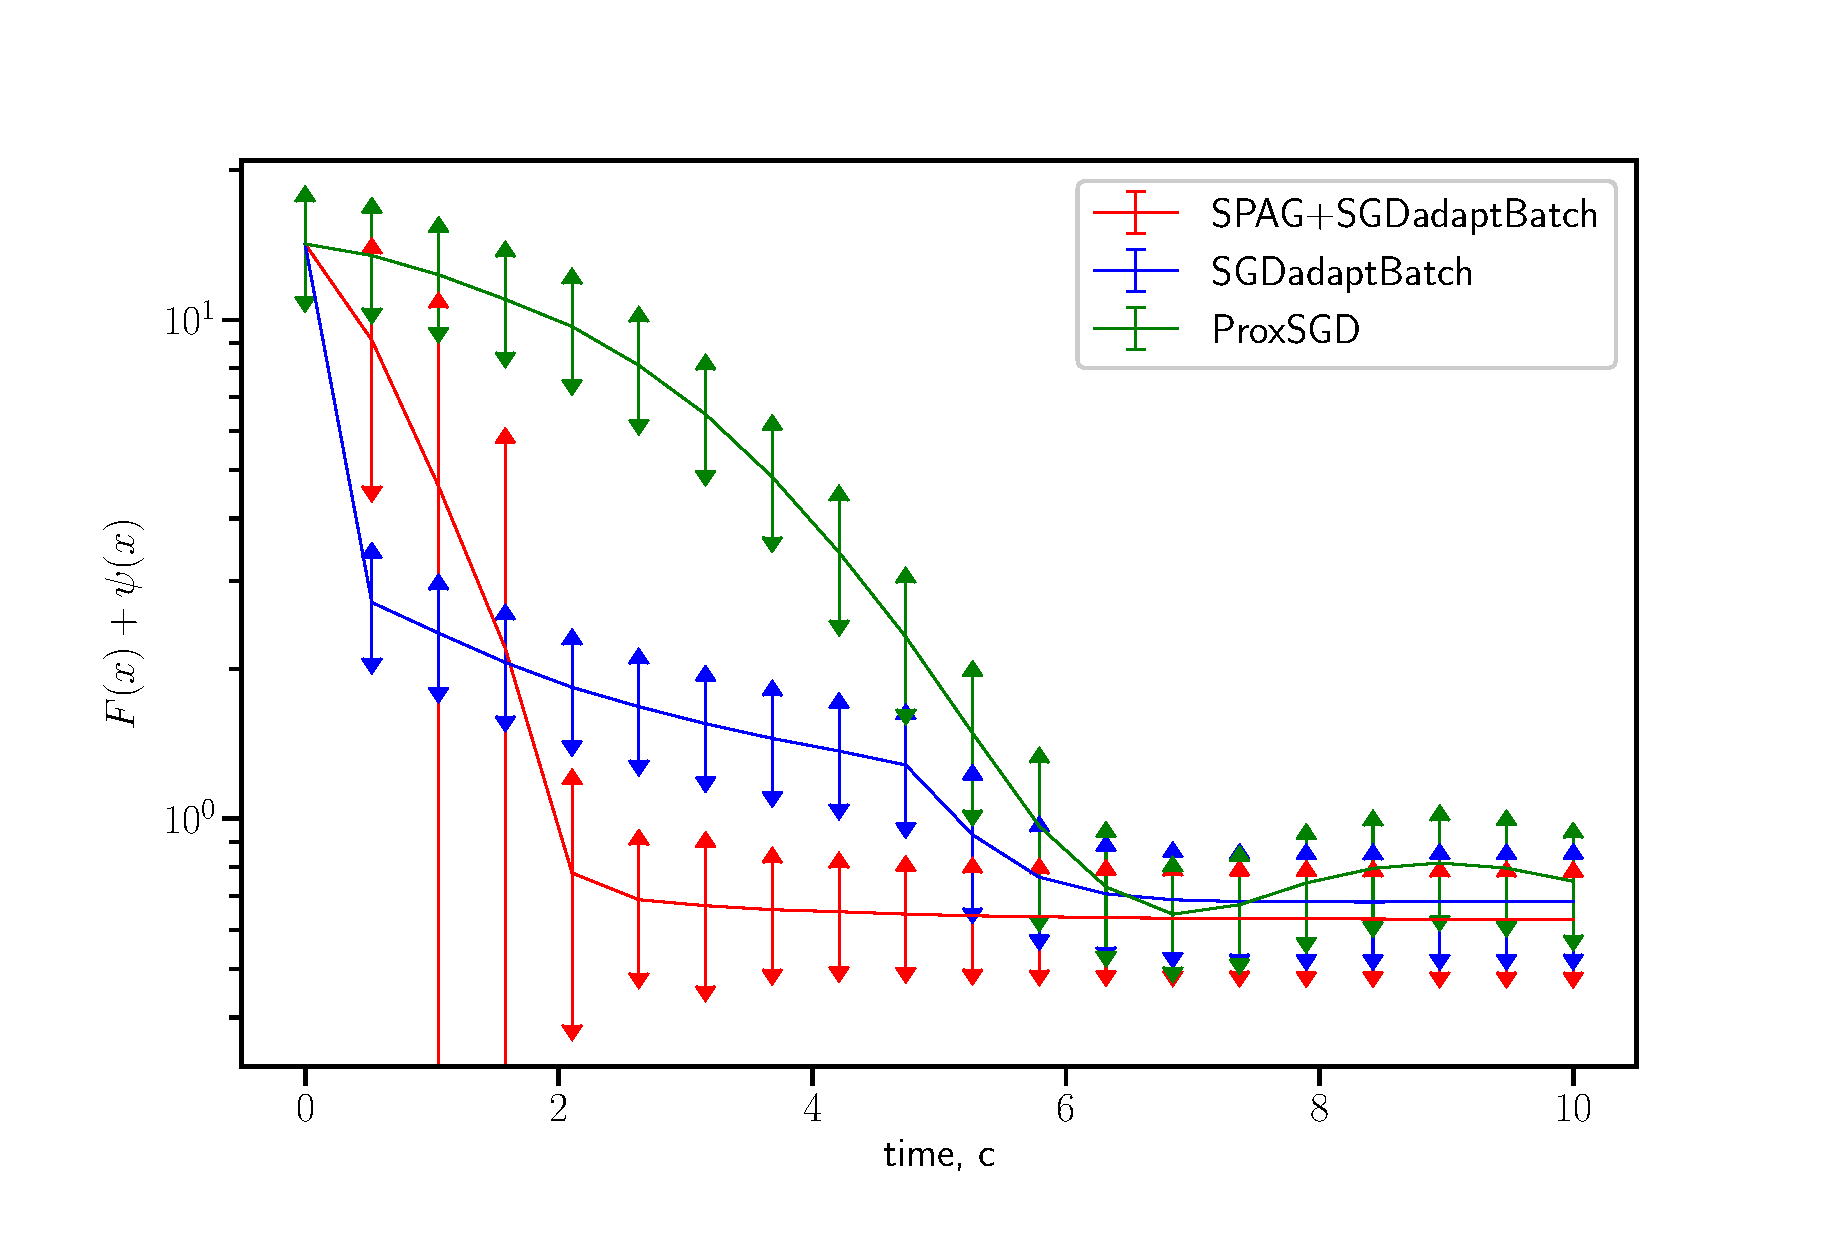
\includegraphics[scale=1]{grafics.eps}}
\label{fig:image}
\end{figure}

\begin{table}[H]
\centering
%\resizebox{\columnwidth}{!}
\end{table}

\medskip
\hrule\medskip
\Head{Conclusion}\\
The SPAG method showed a high rate of convergence, but its advantage became noticeable only at large matrix dimensions. In addition, the appearance of a subproblem leads to a doubling of the number of hyperparameters of the method and difficulties in configuring them. Moreover, new hyperparameters appear, such as the number of iterations of a submetod or its maximum discrepancy.

\medskip
\hrule\medskip
\Head{Acknowledgements}\\
My thanks are due to teacher Danil Merkulov, curators Alexander Gasnikov, Pavel Dvurechensky and Dima Pasechnyuk.
\vspace{-1.4cm}
\bibliographystyle{unsrt}
\bibliography{biblio2}

\end{textblock}

\end{document}